\documentclass[10pt,a4paper]{article}
\usepackage[a4paper, left=3cm, right=3cm, top=3cm, bottom=3cm, headsep=10mm, footskip=12mm]{geometry}
\usepackage[T1]{fontenc}
\usepackage[ngerman, english]{babel}    % mehrsprachiger Textsatz
% babel: letzte Sprache in Optionen zeigt die Sprache des Dokumentes
% und kann durch den Befehl \selectlanguage{} geaendert werden
% Passen Sie die Optionen des babel-Paketes nach Bedarf an!
\usepackage{float}
\usepackage{graphicx}
\usepackage{url}
\usepackage{pdflscape}
\usepackage{mathtools}
\usepackage{amssymb, amsmath, amstext}
\usepackage{amsthm}
\usepackage{xcolor}
\usepackage{nameref}
\usepackage{siunitx}
\usepackage{makecell}
\usepackage{hyperref}
\usepackage{enumitem}
\usepackage[superscript,biblabel]{cite}
\usepackage{caption}
\usepackage{subcaption}
\usepackage{tabularx} 			% Tabellen erzeugen
\usepackage{multirow}			 % Zeilen in Tabellenbearbeitung
\usepackage{multicol} 			% Spalten in Tabellenbearbeitung 
\usepackage{lmodern}                        % Ersatz fuer Computer Modern-Schriften 
\usepackage{amsmath}                                           % zum besseren Aussehen am Bildschirm
\usepackage{booktabs} % für schönere Tabellen
\usepackage{sidecap}
\usepackage{rotating} % für die Landscape-Umgebung
\usepackage{afterpage}
\definecolor{Bluetitle}{HTML}{1F3864}
\definecolor{softbluetitle}{HTML}{274D7E}
\definecolor{Greyish}{HTML}{5A5A5A}
\renewcommand{\refname}{Reference}
\usepackage{array,multirow}
\newcommand{\specialcell}[2][c]{%
	\begin{tabular}[#1]{@{}c@{}}#2\end{tabular}}




\begin{document}
	
	\begin{titlepage}
		\begin{center}
			\begin{figure}[h!tbp]
				
\includegraphics[width=\linewidth]{HUlogo.PNG}
			\end{figure}
			\vspace*{2 cm}
			
			\textcolor{Bluetitle}{\textbf{\huge Atmung und Gärung}}\par
			
			\vspace*{2cm}
			
			\textcolor{Greyish}{\textbf{Versuchsdurchführende}}\par
			\textcolor{Greyish}{Oscar Moore (634083)}\par
			\textcolor{Greyish}{Fridolin Rehnig (625757)}\par
			\textcolor{Greyish}{Philipp Kunze (625468)}\par
			\textcolor{Greyish}{Daniel Kollenkirchen (625426)}\par
			\textcolor{Greyish}{Huyen Anh Nguyen (572309)}\par
			
			\vspace*{0.5cm}
			\textcolor{Greyish}{\textbf{Versuchsort}}\par
			\textcolor{Greyish}{Campus Nord, Haus 9}\par
			\textcolor{Greyish}{R2006}\par
			\vspace*{0.5cm}
			\textcolor{Greyish}{\textbf{Versuchsbetreuer}}\par
			\textcolor{Greyish}{Dr. Christina Kühn}\par
			
			\vspace*{2 cm}
			
			\textcolor{Greyish}{09. Juli 2024}\par
			
			
			
			
		\end{center}
	\end{titlepage}
	
	\tableofcontents
	
	\section{Einführung}	
		Bei der Photosynthese gibt es zwei Hauptmechanismen der CO$_2$-Fixierung, welche jeweils von entweder C3- oder C4-Pflanzen genutzt werden und korrespondieren mit der unterschiedlichen Stärkesynthese, bzw. -akkumulierung.
		Zu den C3-Pflanzen zählen mehr als 90 $\%$ der höheren Pflanzen und diese fixieren CO$_2$ direkt im Calvin-Zyklus, im Mesophyll. In diesem Prozess wird CO$_2$  zuerst, durch das Enzym RuBisCO, in Ribulose-1,5-bisphosphat fixiert, wodurch Glycerat-3-Phosphat (3 C-Atome) entsteht, welches über mehrere Triosephosphate reduziert wird und als Vorläufer für Stärke dienen. Die Stärke wird tagsüber, als ein Produkt der lichtgetriebenen Photosynthese, im Mesophyll synthetisiert und gespeichert. Nachts hingegen wird Stärke, durch Hydrolyse, zu Glucose und Maltose abgebaut, welche aus den Chloroplasten in das Cytosol transportiert werden und dort in Saccharose umgewandelt werden, welches über das Phloem, nach der source-to-sink-Methode in andere Teile der Pflanze transportiert wird. Der Mechanismus der C3-Pflanzen ist bei hohen Temperaturen und niedrigen CO$_2$-Konzentrationen ineffizient, da die RuBisCO auch eine Oxygenase-Aktivität aufweist, was zur unerwünschten Photorespiration führt. \\
		Im Gegensatz dazu haben C4-Pflanzen einen alternativen Mechanismus entwickelt, der es ihnen ermöglicht, auch unter stressigen Umweltbedingungen effizient Photosynthese zu betreiben: die räumliche Trennung der Photosynthese und CO$_2$ -Fixierung. Die primäre CO$_2$-Fixierung findet im Mesophyll statt und von der PEP-Carboxylase durchgeführt, wobei das CO$_2$  in Phosphoenolpyruvat (PEP) fixiert wird und Oxalacetat (4 C-Atome) gebildet wird. Diese wird in Malat umgewandelt und in die Bündelscheidenzellen transportiert, wo es wiederum decarboxyliert wird, um CO$_2$ freizusetzen – dieses wird im Calvin-Zyklus weiterverarbeitet, unter anderem zu Stärke, welches auch in den Bündelscheidenzellen gespeichert wird. Der Abbau erfolgt wie bei C3-Pflanzen. Durch räumliche Trennung wird, bei C4-Pflanzen die Photorespiration verringert und die Effizienz der Photosynthese erhöht. Zudem hat die PEP-Carboxylase eine höhere CO$_2$ -Affinität und kann dieses deshalb auch bei geringeren Konzentrationen fixieren. \\
		\\
		Im 1. Versuch wird die unterschiedliche Stärkeakkumulation, mithilfe von Stärkefärbung, von Tabakpflanzen, C3-Pflanzen, und Maispflanze, C4-Pflanzen analysiert. Zudem werden beide Pflanzenarten auf anatomische Unterschiede in den Leitbündeln und Chloroplasten untersucht. Ziel des Experiments ist es, mithilfe der Analyse dieser Unterschiede, die physiologischen und anatomischen Besonderheiten der beiden Pflanzentypen besser zu verstehen. \\
		Die Grundlage der Stärkefärbung liegt in der molekularen Struktur: Stärke besteht aus Amylose und Amylopektin. Amylose und Amylopektin sind beide Polymere, bestehend aus Glukose-Untereinheiten, Ersteres ist verzweigt und Zweiteres linear. Hierbei steht jede Glucose-Untereinheit in der Kette steht zur nächsten in einem durch die glykosidische Bindung bestimmten Winkel. Das führt dazu, dass Amylose-Polymere eine regelmäßige helikale Struktur annehmen. Die Zugabe von Iod führt zu einer charakteristischen blau-schwarzen Färbung der Stärke, da die Iodmoleküle sich an unpolare Gruppen in den Hohlräumen der unverzweigten Amylose anlagern und die helikale Struktur des Moleküls stabilisieren. \\
		\\
		Im 2. Versuchsteil wird die physiologische Bedeutung des Saccharosetransporters SUT1 in Tabakpflanzen (Nicotiana tabacum) untersucht. Hierbei werden zuerst, die Glucose-, Fructose- und Saccharose-Gehalte in den Blättern der Saccharosetransporter-Antisense-Pflanzen untersucht und dann, die Stärkeverteilung in abgedunkelten Blättern von einem Tabak-Wildtyp und einer Saccharosetransporter-Antisense-Pflanze verglichen.\\
		Saccharosetransporter sind essentielle Proteine für den Langstreckentransport von Photoassimilaten, wie Saccharose, innerhalb der Pflanze. Sie spielen eine Schlüsselrolle bei der Phloembeladung und dem Transport von Nährstoffen von dem source-Gewebe zum sink-Gewebe. Um die Funktion des SUT1-Transporters zu untersuchen, werden transgene Tabakpflanzen verwendet. Genauer werden die Produktion von RNA-Molekülen initiiert, die komplementär zur mRNA des Zielgens sind, was die Translation des entsprechenden Proteins hemmt. In diesem Fall wird der Saccharosetransporter SUT1 in den transgenen Pflanzen herunterreguliert. Dadurch können sämtliche physiologische Veränderungen beobachten werden: die Pflanzen zeigen eine stark reduzierte Wachstumsrate, Veränderungen in Blättern, Wurzeln und Speicherorganen im Vergleich zu Kontrollpflanzen. Diese Veränderungen unterstreichen die wichtige Rolle des SUT1-Transporters im Kohlenhydratstoffwechsel und -transport.
	
	\section{Material und Methode}

	
	\section{Ergebnis}
	
	\subsection{Wildtyp vs Antisense}
		Zuerst wurden die Extinktionen der Eichreihe mit den bekannten  Glukose-Lösungen bestimmt, um eine Eichgerade zu generieren mittels der man den Glukosegehalt der unbekannten Lösung, sowie der Wildtyp- und Antisense Extrakte ermitteln kann. Daraufhin wurden ebenfalls die Extinktionen der Extrakte und der unbekannten Probe gemessen. Es wurde jede Probe immer doppelt angesetzt und gemessen und daraus der Mittelwert gebildet, um mögliche Fehlerwerte zu minimieren. Bei der Bestimmung der unbekannten Probe und der Extrakte, wurde die Extinktion vor Zugabe der Hexokinase und 15 minuten nach der Zugabe bestimmt und nach Gleichung \ref{eq:delta E} berechnet. Die Glukosemenge lies sich dann durch die Steigung der Eichgeraden und den berechneten Extinktionswerten nach Gleichung (2) errechnen. Dabei zeigte die unbekannte Probe den mit Abstand höchsten Glukosegehalt mit ca. 19$\mu g$. Das Antisense Extrakt wies eine deutlich höhere Glukosemenge, von ca. 7,4$\mu g$ auf, als das Wildtyp Extract mit ca. 4,4$\mu g$. 
		
		
		\begin{equation}\label{eq:delta E}
			\overline{E_2} - \overline{E_1}=\Delta E
		\end{equation}
		\begin{equation}\label{eq: eichkurve}
			\Delta E = a \cdot m \leftrightarrow m=\frac{\Delta E}{a}
		\end{equation}
		\begin{figure}[H]
			\centering
			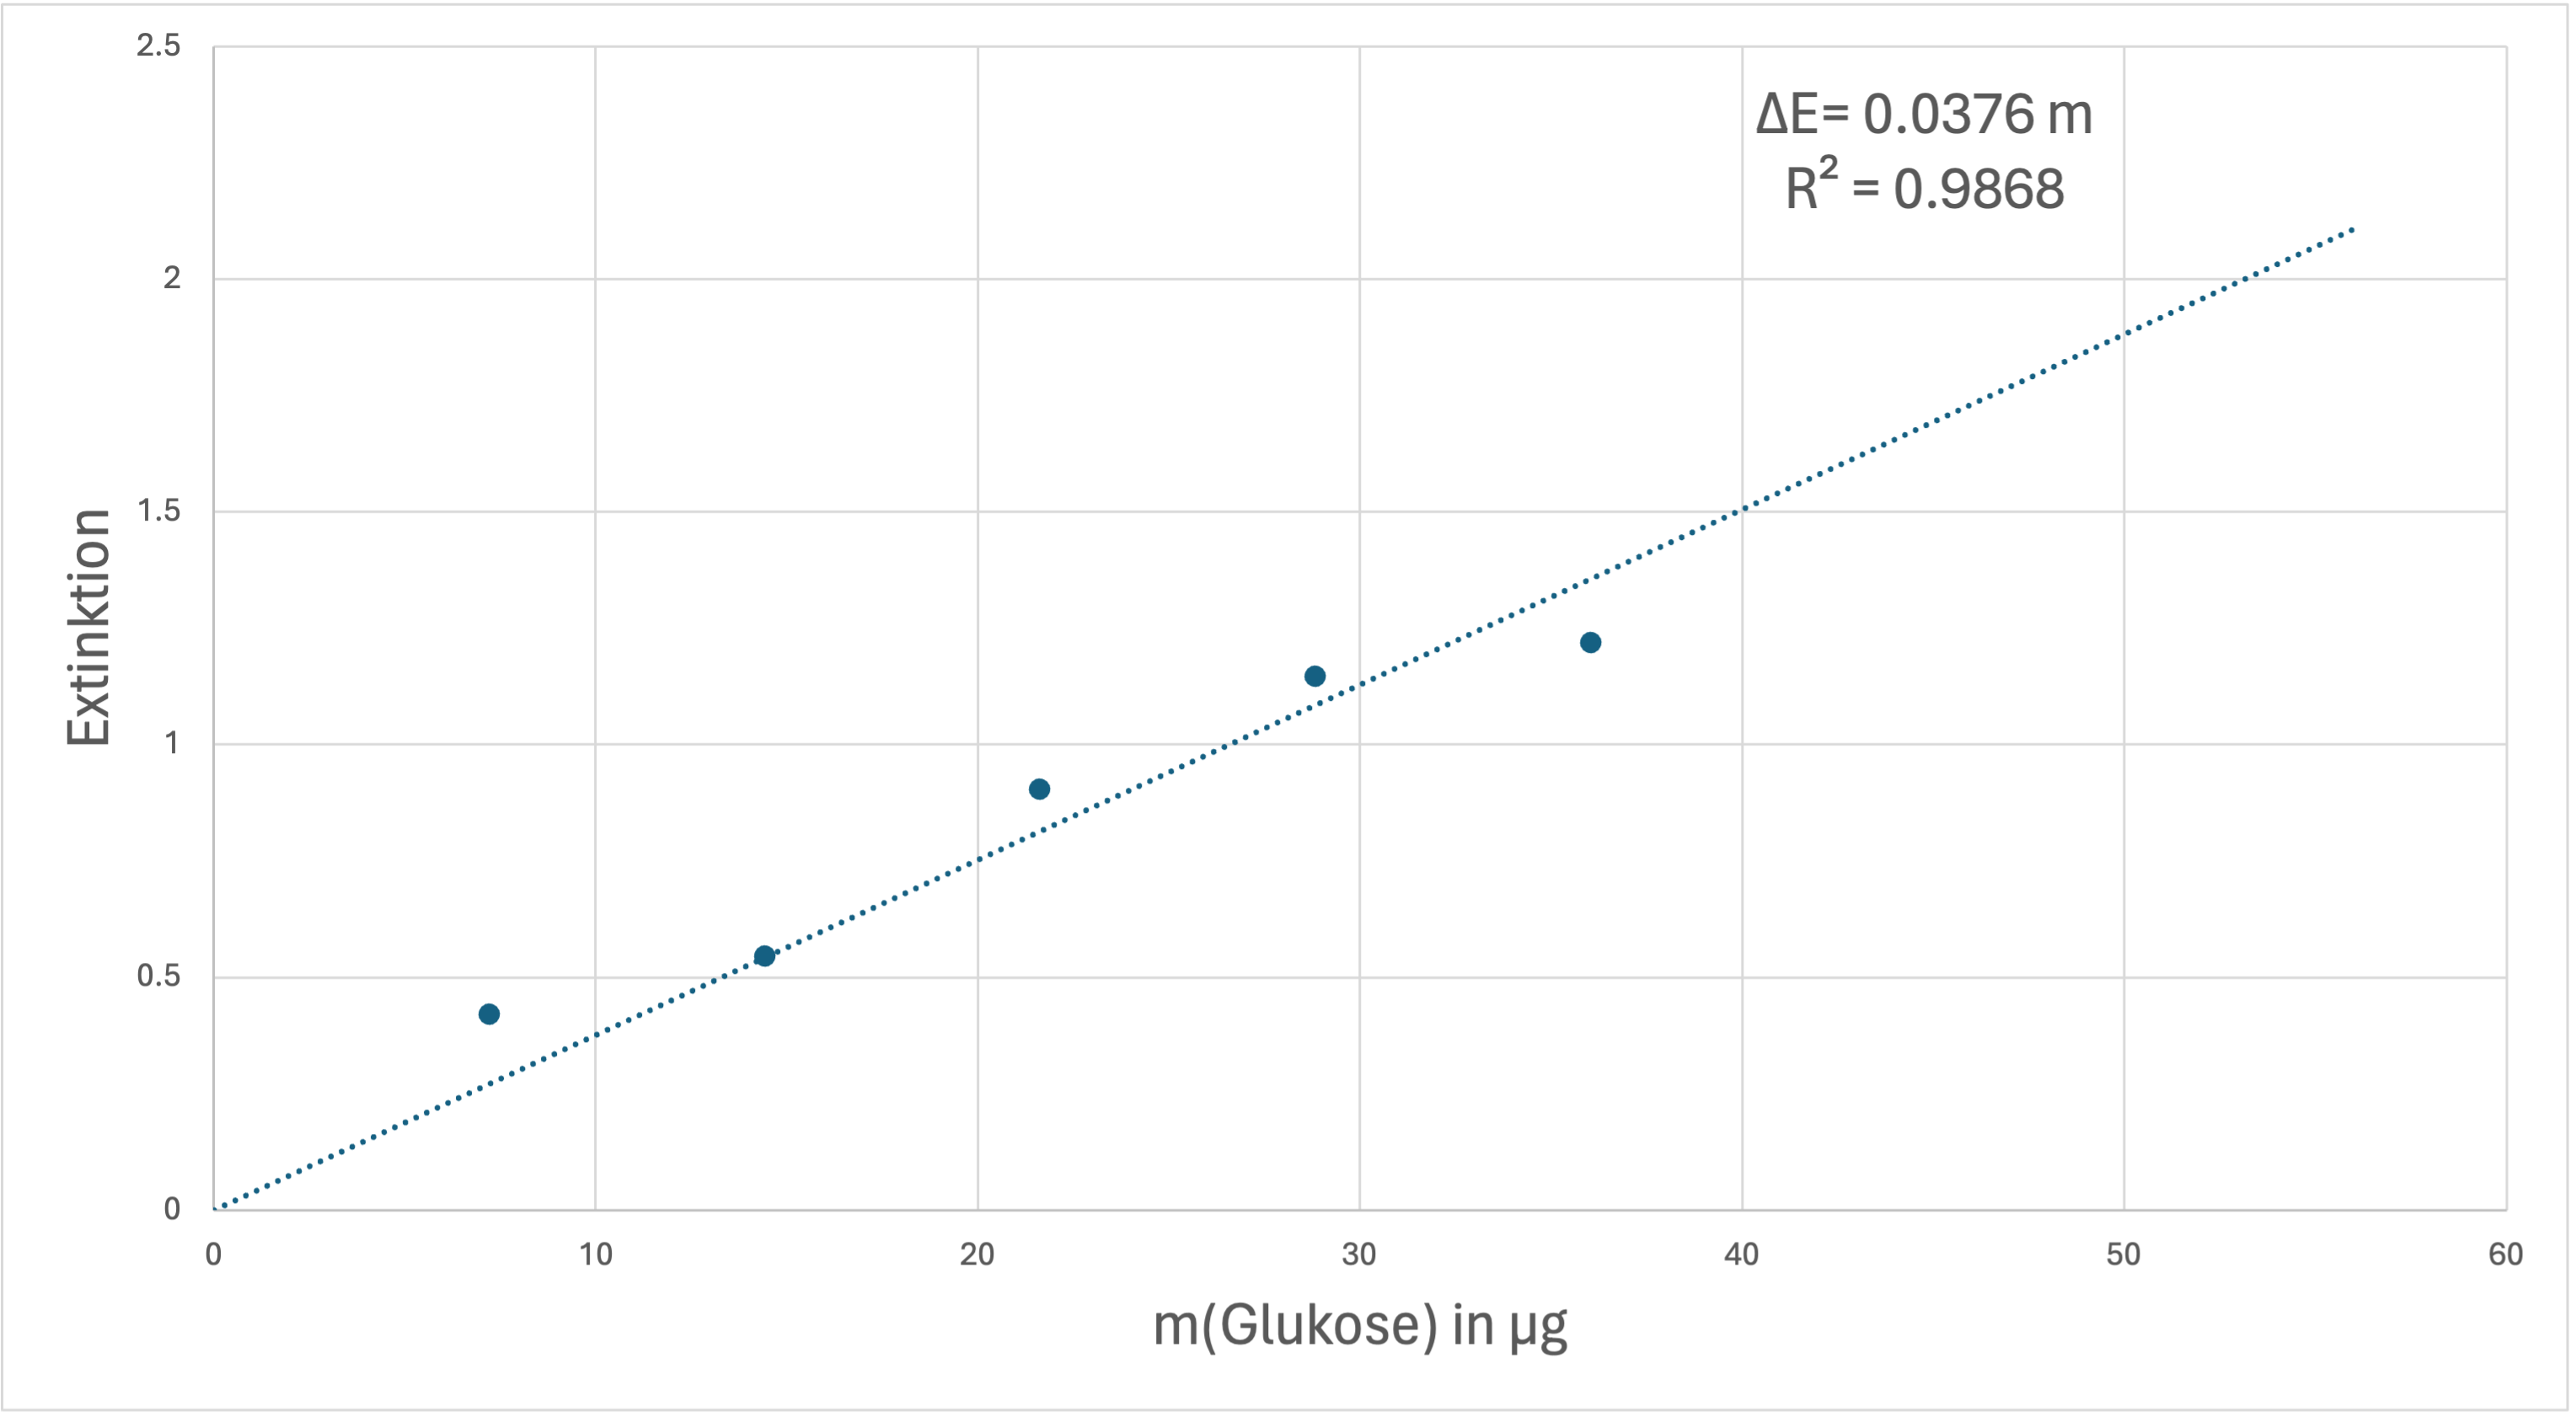
\includegraphics[width=0.75\linewidth]{Eichgerade.png}
			\caption{Eichgerade}
			\label{Abbildung 1}
		\end{figure}
		
		\begin{table}[H]
			\centering
			\begin{tabular}{c|c|c}
				& Glukosemenge in $\mu$g & Glukosemenge in $\mu$g pro mg Frischgewicht\\ 
				\hline
				WT & 4,428191489 & 1,229029001\\
				\hline
				Antisense & 7,380319149 & 2,048381668\\
				\hline
				Unbekannt & 19,02925532 & -\\
			\end{tabular}
			\caption{Zusammenfassung der Ergebnisse}
			\label{tab:my_label}
		\end{table}
	
	\section{Diskussion}

	\section{Anhang}
	\subsection{Rohdaten}


	
\end{document}